\subsection{Unit test}
Nell'iterazione 3 è stata testata la funzione findById() della classe ReservationRepository.

\begin{lstlisting}
@DataJpaTest
class ReservationRepositoryTest {

        @Autowired
        private ReservationRepository underTest;

        @Test
        void findById() {

                //given
                Date date = new Date(100);
                Reservation expected = new Reservation(1, date, new Boolean(true));
                underTest.save(expected);

                //when
                Reservation result = underTest.findById(expected.getId()).get();

                //then
                assertEquals(expected.getId(), result.getId());
        }
}
\end{lstlisting}

\begin{figure}[h!]
\begin{center}
  % Requires \usepackage{graphicx}

   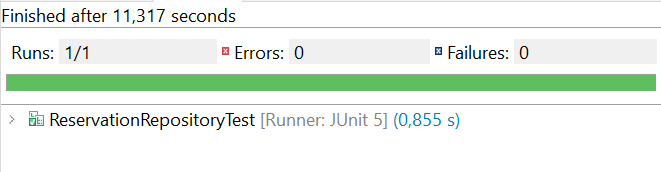
\includegraphics[width=16cm]{Iterazione 3/test/unit test/test.PNG}\\
  \caption{findById()}
\end{center}
\end{figure}
